% vim:encoding=utf8 ft=tex sts=2 sw=2 et:

\documentclass{classrep}
\usepackage[utf8]{inputenc}
\usepackage{fixltx2e}
\usepackage{url}
\usepackage{graphicx}
\usepackage{siunitx}


\studycycle{Informatyka, studia niestacjonarne, inż I st.}
\coursesemester{VI}

%\coursename{hhhhhhhheoretyczna i stosowana}
\coursename{Inteligentna Analiza Danych}
\courseyear{2013/2014}

\courseteacher{mgr inż. Michał Pryczek}
\coursegroup{sobota, 11:15}

\author{
  \studentinfo{Łukasz Ochmański}{183566} \and
  \studentinfo{Przemysław Szwajkowski}{173524}
}

\title{Zadanie 2a: Perceptron Wielowarstwowy}
\svnurl{http://iad-lukasz-ochmanski.googlecode.com/svn/trunk/02}

\begin{document}
\maketitle


\section{Cel}
Celem zadania było zaimplementowanie programu umozliwiajacego tworzenie
perceptronu wielowarstwowego (ang. Multi-Layer Perceptron, w skrócie:
MLP) oraz wsteczna propagacje błedów jako metode jego nauki. Kolejnym
etapem zadania było wykorzystanie aplikacji w celu stworzenia perceptronu
o podanej architekturze(4:2:4) oraz wykonanie na nim zadanych
eksperymentów.

\section{Wstęp}
Podstawowym elementem sieci jest neuron. Do kazdego neuronu dochodzi
dowolna ilosc wejsc, natomiast wyjscie neuronu jest tylko jedno. Dodatkowo
dla kazdego wejscia neuronu, przypisana jest waga w naszym przypadku losowana
z zakresu -0.5 - 0.5. Kolejnym elementem jest Bias, czyli tzw wejscie
obciazajace majace zawsze wartosc 1 któremu równiez przypisana jest waga.
Neurony grupowane sa w warstwy, gdzie w przypadku dwóch sasiadujacych
ze soba warstw wyjscia wszystkich neuronów jednej warstwy trafiaja jako
wejscia neuronów warstwy nastepnej. Wyrózniamy trzy rodzaje warstw :
1. Warstwa wejsciowa - zawsze jedna.
2. Warstwa ukryta - wiele.
3. Warstwa wyjsciowa - zawsze jedna.
\\*

\begin{figure}[ht]
\centering
			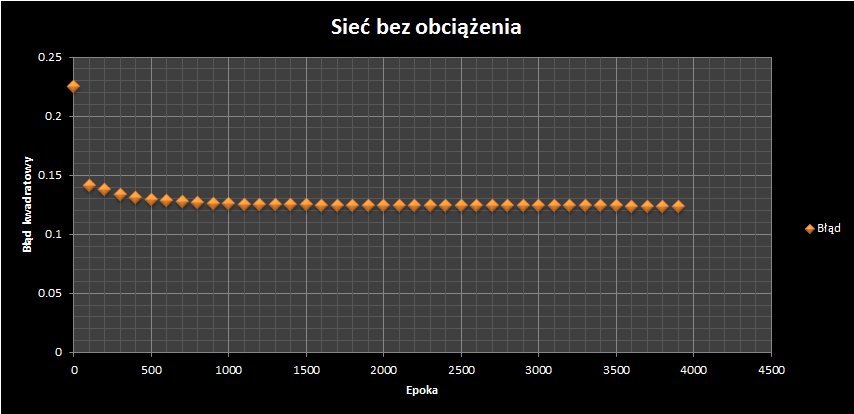
\includegraphics[scale=0.65]{pictures/test01.png}
	\caption{Siec bez obciazenia}
	\label{fig:Siec bez obciazenia}
\end{figure}

Jak widać na wykresie nr 1 siec bez obciążenia zatrzymuje się na poziomie błędu: 0.123873369,
co jest dość słabym rezultatem.


\begin{figure}[ht]
\centering
			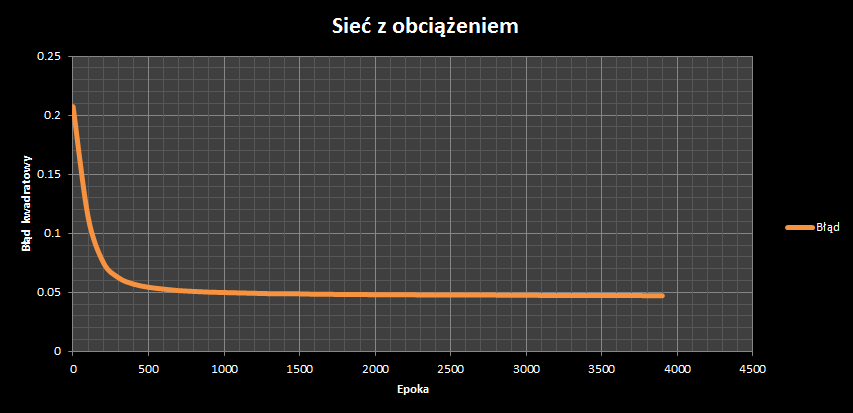
\includegraphics[scale=0.65]{pictures/test02.png}
	\caption{Siec z obciazeniem}
	\label{fig:Siec z obciazeniem}
\end{figure}

Na wykresie 2 zaprezentowana wyniki nauki dla sieci z obciążeniem. Rezultat jest ponad trzykrotnie lepszy: 0.04719184


\begin{figure}[ht]
\centering
			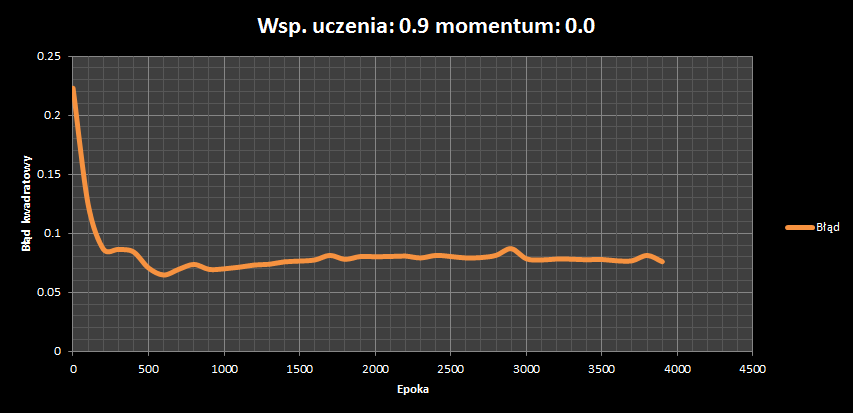
\includegraphics[scale=0.65]{pictures/test03.png}
	\caption{Siec ze wspolczynnikiem nauki 0.9}
	\label{fig:Siec ze wspolczynnikiem nauki 0.9}
\end{figure}

Na wykresie 3: Sieć bez momentum i przy wysokim współczynniku nauki: 0.9 zatrzymała się na wartości błędu: 0.07603583


\begin{figure}[ht]
\centering
			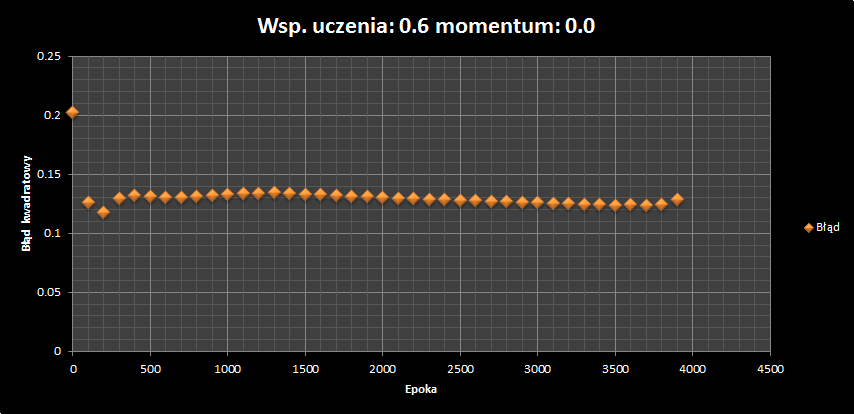
\includegraphics[scale=0.65]{pictures/test04.png}
	\caption{Siec ze wspolczynnikiem nauki 0.6}
	\label{fig:Siec ze wspolczynnikiem nauki 0.6}
\end{figure}

Na wykresie 4: Sieć bez momentum i przy współczynniku nauki: 0.6 osiągnęła nieco gorszy rezultat niż sieć w poprzednim przykładzie. Sieć zatrzymała się na wartości błędu: 0.128971259

\begin{figure}[ht]
\centering
			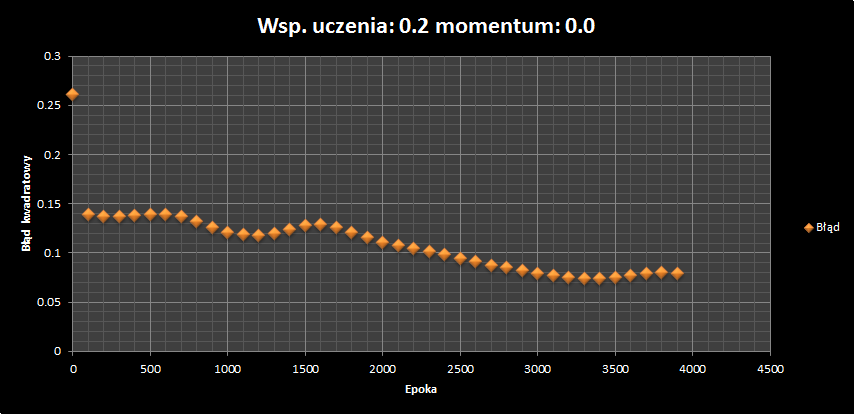
\includegraphics[scale=0.65]{pictures/test05.png}
	\caption{Siec ze wspolczynnikiem nauki 0.2}
	\label{fig:Siec ze wspolczynnikiem nauki 0.2}
\end{figure}

Na wykresie 5: Sieć ze współczynnikiem nauki 0.2 osiągnęła wyniki lepsze niż na wykresie nr 3: 
0.079574248. 

\begin{figure}[ht]
\centering
			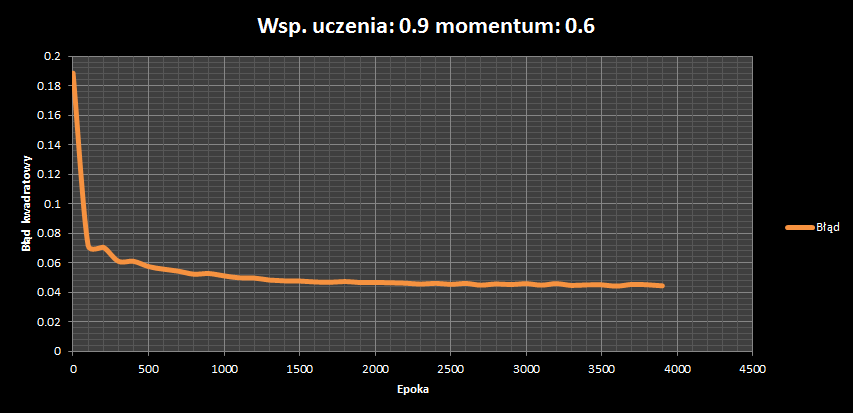
\includegraphics[scale=0.65]{pictures/test06.png}
	\caption{Siec z momentum 0.6}
	\label{fig:Siec z momentum 0.6}
\end{figure}

Na wykresie 6: Sieć z wysokim wpółczynnikiem i umiarkowanym momentum 0.6 osiągnęła najlepszy wynik wśród zaprezentowanych: 0.04446939


\begin{figure}[ht]
\centering
			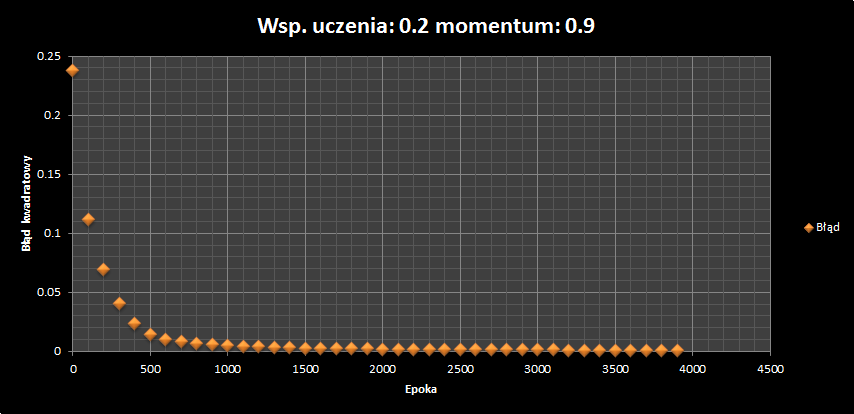
\includegraphics[scale=0.65]{pictures/test07.png}
	\caption{Siec z momentum 0.9}
	\label{fig:Siec z momentum 0.9}
\end{figure}

Na wykresie 7: Sieć z wysokim momentum osiągnęła nieco słabszy rezultat niż ta z niższym momentum: 0.066697569




\begin{thebibliography}{0}
  \bibitem{l2short} \textsl{Ryszard Tadeusiewicz} - Sieci neuronowe, \textsl{Wyd. 2., Warszawa 1993}
  \bibitem{l2short} ``Learning and neural networks'' [\url{http://en.wikiversity.org/wiki/Learning_and_neural_networks}]
  \bibitem{l2short} UCI Machine Learning Repository \textsl{Iris Data Set}
\end{thebibliography}
\end{document}